% % Chapter 2

\chapter{对凸多边形进行三角化}

\section{概述}
凸多边形\footnote{每个内角均小于\(180°\)的多边形}是平面多边形中最简单最易处理的一类。
定义一个多边形S 满足
对于一个凸多边形\(S\),存在多种方案将其分割为n-2个三角形。其中Delaunay划分可以生成满足最小角最大特性,细长三角形较少的优秀划分方案。

\section{朴素的划分方案}

由于凸多边形的性质,多边形任意两个顶点之间连边均在多边形内部。因此最简单的划分方案即为 对于\(i\in [2,n-2]\),沿边\(S_0,S_i\)进行一次分割,即可产生总共n-2个三角形。该方案最为简便,且产生的三角形均有一个共同顶点,但产生的三角形形状均为细长型,相对形态较劣。

\section{改进的朴素划分}

由于对凸多边形分割后产生的两个多边形仍为凸多边形,我们可以采用分治法来一定程度的优化上述方案。
一种可行的方案如下:
\begin{itemize}
    \item 若当前多边形为三角形则结束算法;
    \item 随机选择两个不相邻的顶点连边,将当前多边形分割为两部分;
    \item 对分割出的两个子多边形调用本算法进行分割,并将分割的结果加入答案。
\end{itemize}

该方案仍然有较大优化空间,例如选择点对进行分割时可以选择多边形较短的轴进行切割以使两部分更加规整,但实际应用中优化意义不甚显著,且计算复杂度大幅增加。

\section{完美三角剖分}
Delaunay triangulation(简称DT)是一种三角剖分方式,其结果满足以下性质:
\begin{itemize}
    \item 对于三角剖分中产生的每一个三角形,其外接圆中不包含点集V中的其他点。
    \item 若对点集的三角剖分结果中每一个三角形的最小角升序排列,则DT所得到的数值比其他三角剖分的数值大。
    \item 若点集中任意四点均不共圆,则产生的三角剖分唯一。
\end{itemize}

\begin{figure}[htbp]
    \centering
    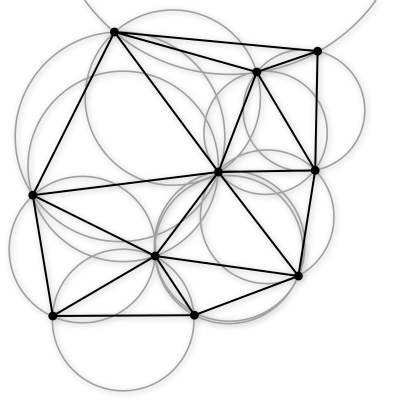
\includegraphics[width=0.4\textwidth]
    {figures/triangulation-1.png}
    \caption{DT示例}
\end{figure}

若进行三角剖分的点集中存在四点共圆,虽然计算其Delaunay triangulation时得到的结果不唯一,但仍不破坏其余性质。由于最小角最大的特性,DT可以产生理论最优的划分。而根据三角剖分的性质,对凸多边形顶点点集进行三角剖分所得到的三角形集合即为待求的三角化结果。

一种利用分治思想在\(O(n\log n)\)复杂度内计算点集的Delaunay triangulation方法如下:

首先将给定点集按照 x 坐标升序排列,如图~\ref*{DT1}所示。

\begin{figure}[htbp]
    \centering
    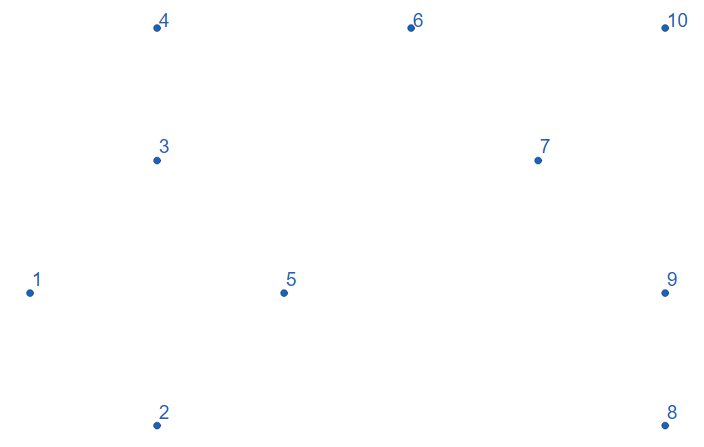
\includegraphics[width=0.5\textwidth]
    {figures/DT1.png}
    \caption{排好序的大小为10的点集}
    \label{DT1}
\end{figure}
\newpage
一旦点集有序,我们就可以不断地将其平分成两个部分,直到子点集大小不超过 3。然后这些子点集可以立刻剖分为一个三角形或线段。

\begin{figure}[htbp]
    \centering
    \begin{minipage}{0.4\textwidth}
        \centering
        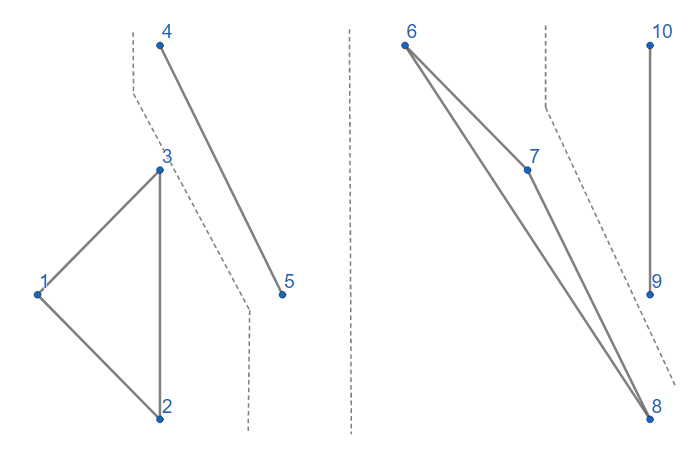
\includegraphics[width=\textwidth]
        {figures/DT2.png}
        \caption{分治为包含2或3个点的点集}
    \end{minipage}
    \begin{minipage}{0.4\textwidth}
        \centering
        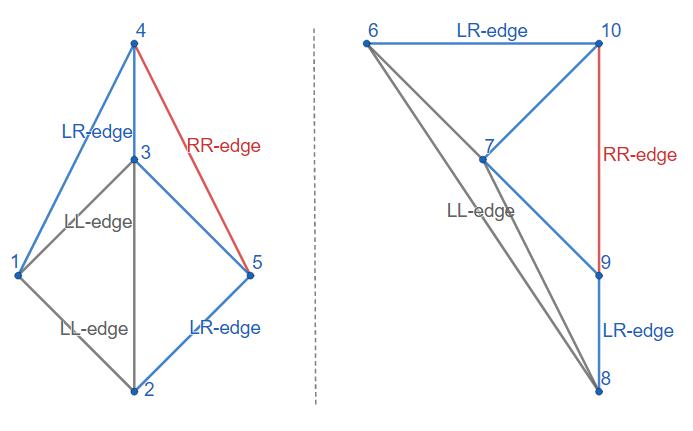
\includegraphics[width=\textwidth]
        {figures/DT3.png}
        \caption{三种不同的边}
        \label{DT3}
    \end{minipage}
\end{figure}

在分治回溯的过程中,已经剖分好的左右子点集可以依次合并。合并后的剖分包含 LL-edge(左侧子点集的边)。RR-edge(右侧子点集的边),LR-edge(连接左右剖分产生的新的边),如图~\ref*{DT3} LL-edge(灰色),RR-edge(红色),LR-edge(蓝色)。对于合并后的剖分,为了维持 DT 性质,我们可能需要删除部分 LL-edge 和 RR-edge,但我们在合并时不会增加 LL-edge 和 RR-edge。


合并左右两个剖分的第一步是插入 base LR-edge,base LR-edge 是最底部的不与任何LL-edge 及 RR-edge 相交的 LR-edge。


然后,我们需要确定下一条紧接在base LR-edge 之上的 LR-edge。比如对于右侧点集,下一条 LR-edge 的可能端点(右端点)为与 base LR-edge 右端点相连的 RR-edge 的另一端点(6, 7, 9 号点),左端点即为 2 号点。
\begin{figure}[htbp]
    \centering
    \begin{minipage}{0.4\textwidth}
        \centering
        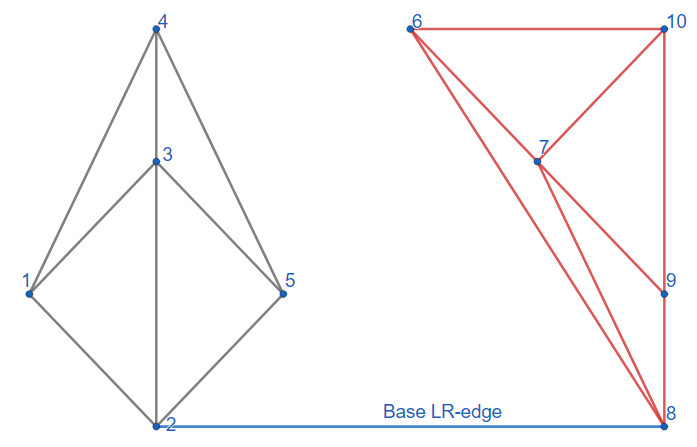
\includegraphics[width=\textwidth]
        {figures/DT4.png}
        \caption{合并左右剖分}
    \end{minipage}
    \begin{minipage}{0.4\textwidth}
        \centering
        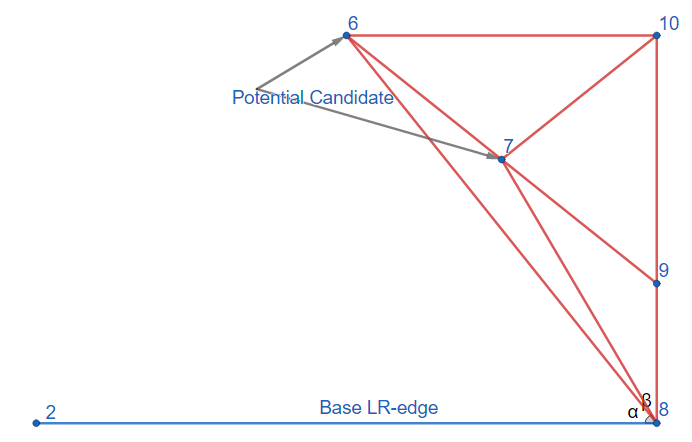
\includegraphics[width=\textwidth]
        {figures/DT5.png}
        \caption{下一条LR-edge的可能位置}
    \end{minipage}
\end{figure}

对于可能的端点,我们需要按以下两个标准检验:

\begin{enumerate}
    \item 其对应 RR-edge 与 base LR-edge 的夹角小于 180 度。即,新选择的端点在当前base LR-edge的“上方”。
    \item base LR-edge 两端点和这个可能点三点构成的圆内不包含任何其它可能点。
\end{enumerate}

如图~\ref*{DT6},6 号可能点所对应的绿色圆包含了 9 号可能点,而 7 号可能点对应的紫色圆则不包含任何其它可能点,故 7 号点为下一条 LR-edge 的右端点。

对于左侧点集,我们做镜像处理即可。

当左右点集都不再含有符合标准的可能点时,合并即完成。当一个可能点符合标准,一条 LR-edge 就需要被添加,对于与需要添加的 LR-edge 相交的 LL-edge 和 RR-edge,将其删除。

当左右点集均存在可能点时,判断左边点所对应圆是否包含右边点,若包含则不符合;对于右边点也是同样的判断。在未出现四点共圆的情况下每次只会有一个可能点符合标准,否则任选其一即可。

\begin{figure}[htbp]
    \centering
    \begin{minipage}{0.32\textwidth}
        \centering
        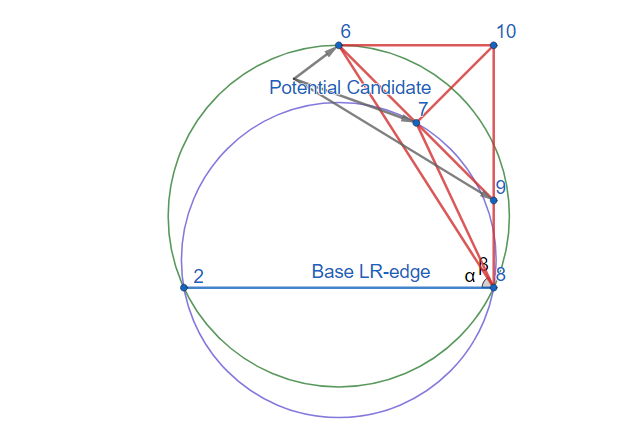
\includegraphics[width=\textwidth]
        {figures/DT6.png}
        \caption{检验可能点}
        \label{DT6}
    \end{minipage}
    \begin{minipage}{0.32\textwidth}
        \centering
        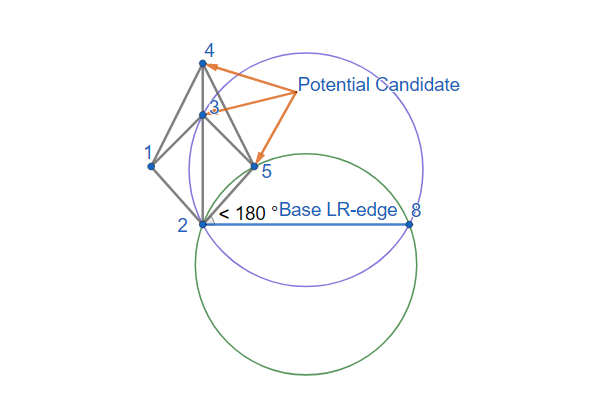
\includegraphics[width=\textwidth]
        {figures/DT7.png}
        \caption{镜像处理另一半点集}
    \end{minipage}
    \begin{minipage}{0.32\textwidth}
        \centering
        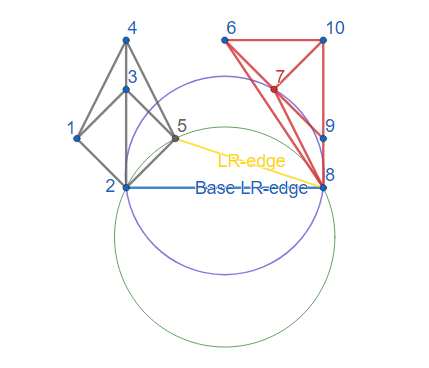
\includegraphics[width=\textwidth]
        {figures/DT8.png}
        \caption{下一条LR-edge}
    \end{minipage}
\end{figure}



重复以上步骤即可完成Delaunay triangulation的构建。

由此我们完成了对凸多边形的三角化。
% \section{公式的使用}
% 在文中引用公式可以这么写:$a^2+b^2=c^2$这是勾股定理,他还可以表示为$c=\sqrt{a^2+b^2}$,还可以让公式单独一段并且加上编号。注意,公式前请不要空行。
% \begin{equation}
% \sin^2{\theta}+\cos^2{\theta}=1 \label{eq:pingfanghe}
% \end{equation}

% 还可以通过添加标签在正文中引用公式,如式\eqref{eq:pingfanghe}。

% 我们还可以轻松打出一个漂亮的矩阵:
% \begin{equation}
%   \mathbf{A}=
%   \left[\begin{matrix}
%     1&2&3&4\\
%     11&22&33&44\\
%   \end{matrix}\right] \times
%   \left[\begin{matrix}
%     22&24\\
%     32&34\\
%     42&44\\
%     52&54\\
%   \end{matrix}\right]
% \end{equation}

% 或者多行对齐的公式:
% \begin{equation}
%   \begin{aligned}
%     f_1(x)&=(x+y)^2\\
%           &=x^2+2xy+y^2
%   \end{aligned}
% \end{equation}


% \section{插图的使用}

% \LaTeX 环境下可以使用常见的图片格式:JPEG、PNG、PDF、EPS等。当然也可以使用\LaTeX 直接绘制矢量图形,可以参考pgf/tikz等包中的相关内容。需要注意的是,无论采用什么方式绘制图形,首先考虑的是图片的清晰程度以及图片的可理解性,过于不清晰的图片将可能会浪费很多时间。

% 图示例如下:

% \begin{figure}[!htb]
%   \centering
%   \includegraphics[width=0.3\textwidth]
%   {figures/whulogo.png}\\
%   \caption{插图示例}
%   \label{fig:whu}
% \end{figure}

% \verb|[htbp]|选项分别是此处、页顶、页底、独立一页。\verb|[width=\textwidth]|让图片占满整行,或\verb|[width=2cm]|直接设置宽度。可以随时在文中进行引用,如图~\ref{fig:whu},建议缩放时保持图像的宽高比不变。

% \section{表格的使用}

% 表格的输入可能会比较麻烦,可以使用在线的工具,如~\href{https://www.tablesgenerator.com/}{Tables Generator}~能便捷的创建表格,也可以使用离线的工具,如~\href{https://ctan.org/pkg/excel2latex}{Excel2LaTeX}~支持从Excel表格转换成\LaTeX{}表格。\href{https://en.wikibooks.org/wiki/LaTeX/Tables}{LaTeX/Tables}~上及~\href{https://www.tug.org/pracjourn/2007-1/mori/mori.pdf}{Tables in LaTeX}~也有更多的示例能够参考。

% \subsection{普通表格}
% 下面是一些普通表格的示例:

% \begin{table}[ht]
%   \centering
%   \caption{简单表格}
%   \label{tab:1}
%   \begin{tabular}{|l|c|r|}
%     \hline
%     我是& 一只 & 普通\\
%     \hline
%     的& 表格& 呀\\
%     \hline
%   \end{tabular}
% \end{table}

% \begin{table}[ht]
%   \centering
%   \caption{一般三线表}
%   \label{tab:2}
%   \begin{tabular}{ccc}
%     \hline
%     姓名& 学号& 性别\\
%     \hline
%     张三& 001& 男\\
%     李四& 002& 女\\
%     \hline
%   \end{tabular}
% \end{table}

% \subsection{跨页表格}
% 跨页表格常用于附录(把正文懒得放下的实验数据统统放在附录的表中),以下是一个跨页表格的示例:

% {\centering
%   \begin{longtable}{ccccccccc}
%   \caption{跨页表格示例} \\
%   \toprule
%   1     & 0 & 5  & 1  & 2  & 3  & 4  &  5 & 6 \\
%   \midrule
%   \endfirsthead

%   \multicolumn{1}{l}{接上一页} \\
%   \toprule
%   1     & 0 & 5  & 1  & 2  & 3  & 4  &  5 & 6 \\
%   \midrule
%   \endhead

%   \bottomrule
%   \hline \\
%   \multicolumn{9}{r}{{转下一页}} \\
%   \endfoot

%   \bottomrule
%   \endlastfoot    

%   1     & 0 & 5  & 1  & 2  & 3  & 4  &  5 & 6 \\
%   1     & 0 & 5  & 1  & 2  & 3  & 4  &  5 & 6 \\
%   1     & 0 & 5  & 1  & 2  & 3  & 4  &  5 & 6 \\
%   1     & 0 & 5  & 1  & 2  & 3  & 4  &  5 & 6 \\
%   1     & 0 & 5  & 1  & 2  & 3  & 4  &  5 & 6 \\
%   1     & 0 & 5  & 1  & 2  & 3  & 4  &  5 & 6 \\
%   1     & 0 & 5  & 1  & 2  & 3  & 4  &  5 & 6 \\
%   1     & 0 & 5  & 1  & 2  & 3  & 4  &  5 & 6 \\
%   1     & 0 & 5  & 1  & 2  & 3  & 4  &  5 & 6 \\
%   1     & 0 & 5  & 1  & 2  & 3  & 4  &  5 & 6 \\
%   1     & 0 & 5  & 1  & 2  & 3  & 4  &  5 & 6 \\
%   1     & 0 & 5  & 1  & 2  & 3  & 4  &  5 & 6 \\

%   \end{longtable}
% }

% \subsection{统计表格}
% 要创建占满整个文字宽度的表格需要使用到tabularx,如不需要,使用tabular就行。引用表格与其它引用一样,只需要:表~\ref{tab:3},统计表格一般是三线表形式。

% \begin{table}[ht]
%   \centering
%   \caption{统计数据表格}
%   \label{tab:3}
%   \begin{tabularx}{\textwidth}{CCCC}
%     \toprule
%     序号&年龄&身高&体重\\
%     \midrule
%     1&14&156&42\\
%     2&16&158&45\\
%     3&14&162&48\\
%     4&15&163&50\\
%     \cmidrule{2-4} %添加2-4列的中线
%     平均&15&159.75&46.25\\
%     \bottomrule
%   \end{tabularx}
% \end{table}

% \section{列表的使用}
% 下面演示了创建有序及无序列表,如需其它样式,\href{https://www.latex-tutorial.com/tutorials/lists/}{LaTeX Lists}~上有更多的示例。

% \subsection{有序列表}
% 这是一个计数的列表
%   \begin{enumerate}
%       \item 第一项
%           \begin{enumerate}
%               \item 第一项中的第一项
%               \item 第一项中的第二项
%           \end{enumerate}
%       \item 第二项
%     \begin{enumerate}[label=(\roman*)]
%       \item 第一项中的第一项
%       \item 第一项中的第二项
%     \end{enumerate}
%       \item 第三项
%   \end{enumerate}

% \subsection{不计数列表}
%   这是一个不计数的列表
%   \begin{itemize}
%       \item 第一项
%       \begin{itemize}
%           \item 第一项中的第一项
%           \item 第一项中的第二项
%       \end{itemize}
%       \item 第二项
%       \item 第三项
%   \end{itemize}

% \section{定理的使用}
% \begin{theorem}
%   设向量$\boldsymbol a\neq\boldsymbol 0$,那么向量$\boldsymbol b//\boldsymbol a$的充分必要条件是:存在唯一的实数$\lambda$,使$\boldsymbol b=\lambda \boldsymbol a$。
% \end{theorem}
% \begin{definition}
%   这是一条定义。
% \end{definition}
% \begin{lemma}
%   这是一条引理。
% \end{lemma}
% \begin{corollary}
%   对数轴上任意一点$P$,轴上有向线段$\vec {OP}$都可唯一地表示为点$P$的坐标与轴上单位向量$\boldsymbol e_u$的乘积:$\vec {OP}=u \boldsymbol e_u$。
% \end{corollary}
% \begin{proposition}
%   这是一条性质。
% \end{proposition}
% \begin{example}
%   这是一条例。
% \end{example}
% \begin{remark}
%   这是一条注。
% \end{remark}